\documentclass[11pt,letterpaper]{article}

\usepackage{anonymous-draft}

\hypersetup{pdftitle={Toward Vector-Symbolic and Neurosymbolic Cyber Planning under Adversarial Uncertainty}}

\begin{document}

\drafttitle{Toward Vector-Symbolic and Neurosymbolic Cyber Planning under Adversarial Uncertainty}

\begingroup\fontsize{10}{11.5}\selectfont\setlength{\parindent}{0pt}\textbf{Abstract.} Cyber planning under adversarial uncertainty depends on evidence representations that remain informative when telemetry is incomplete or manipulated. Learning to regenerate and combine such evidence is a key challenge for vector-symbolic and neurosymbolic decision support. We investigate observation-aware graph learning through methods that weight endpoint-sharing relationships by visible-feature availability and compatibility, and encourage consistent representations and predictions across partially observed views. The methodology builds on masked graph autoencoding and separates the roles of neighborhood aggregation, reconstruction, and consistency training. Evaluation uses selected labeled network flows from the public CTU-13 botnet dataset, organized into graphs with chronological capture splits. Experiments compare graph learners, associative representations, contextual predictors, and inexpensive statistical and neural baselines across recorded telemetry, controlled missingness, and feature replacement, supported by matched ablations and GPU resource measurements. Exploratory comparisons show promising improvements in discrimination and probability estimation from observation-aware aggregation, together with greater tolerance of missing measurements. Consistency training offers another route to improving the reference model while retaining its inference architecture. The ablations reveal how aggregation and reconstruction contribute under different observation conditions and clarify the relationship between predictive quality and computational cost. Together, the methods and controlled evaluation provide practical guidance for learning useful cyber representations and a foundation for evidence regeneration in future vector-symbolic and neurosymbolic planning systems.\par\endgroup\vspace{5pt}

\noindent \textbf{Keywords:} graph learning; masked autoencoders; missing data; consistency regularization; network-flow classification; cyber decision support.\par

\section{Introduction}

Cyber decision support depends on representations of evidence whose availability and trustworthiness can vary. A shared endpoint links two network flows, but does not guarantee that their measurements are equally informative or that their labels agree. Uniform neighborhood aggregation may therefore mix poorly observed or incompatible reports. Masked reconstruction offers a different intervention: learning from intentionally removed measurements might improve representations when observations disappear. Whether either intervention improves downstream decisions requires controlled comparisons.\par

The broader motivation is regeneration of incomplete knowledge for cyber course-of-action planning and replanning. Earlier synthetic investigations in this project examined selective hyperdimensional reconstruction, dependency-constrained regeneration, and direct candidate scoring. Their results did not support assuming that structural coherence or additional complexity improves decision regret. The supplement retains those studies separately (Figures S1–S2). Here we study a narrower measurable component: retrospective classification of recorded flows under controlled telemetry corruption. An endpoint graph expresses observed relationships; it is not a symbolic prerequisite graph.\par

We introduce two task-specific variants of a GraphMAE-adapted classifier [1]. EDGE\_GMAE adds a parameter-free rule based on visible-coordinate overlap and discrepancy. CONS\_GMAE changes training through reconstruction and prediction consistency while preserving inference architecture. Our contribution is their explicit formulation and evaluation with matched controls, conventional inexpensive models, uncertainty, and GPU cost measurements. We report observed improvements without claiming confirmed superiority, first-ever graph weighting or consistency, or demonstrated operational replanning.\par

\section{Related Work}

GraphMAE reconstructs masked node attributes and uses latent remasking [1]. Our comparator follows these mechanisms but uses observed-coordinate mean squared error (MSE), rather than the original scaled cosine error; it is an adaptation, not an exact reproduction. GraphMAE2 already combines multiple remasked reconstruction views with latent representation prediction [2]. Consequently, adding consistency to masked graph learning is established in principle.\par

Robust graph learning also precedes this work. Pro-GNN learns graph structure jointly with prediction [3]; structure-aware DropEdge includes feature-dependent edge sampling [4]. Reliability-ranked masking and decoupled reconstruction have been studied directly for graph autoencoders [5]. More recent work emphasizes neighborhood-context consistency, coverage, and potentially useful heterophilic edges [6]. These findings motivate caution: similarity is not equivalent to useful information. Our narrower contribution is deterministic weighting that explicitly excludes unavailable coordinates, combined with leakage-controlled masked pretraining and telemetry-specific comparisons. We do not experimentally reproduce these additional literature methods; they establish lineage and delimit novelty.\par

\section{Observation-Aware Graph Learning}

\subsection{Representation and comparator}

Each chronological window contains up to 32 retained flows. An undirected edge joins flows sharing any observed source or destination endpoint. Each flow supplies fourteen sanitized measurements and fourteen availability indicators. The GMAE comparator uses a width-128, three-layer residual encoder with self/neighbor transformations, layer normalization, and GELU activations. A readout predicts the probability of the retained botnet label. Five pretraining epochs independently mask 30\% of valid nodes, replace their input with a learned token, remask their latent representation, and reconstruct attributes through a neighbor-propagating decoder. Reconstruction MSE covers only originally observed coordinates of additionally masked real nodes.\par

Supervised training averages binary cross-entropy plus Brier loss over valid flows within each window. Inverse capture-window-frequency weights give training captures equal expected contribution. DENSE has the same architecture without masked pretraining. Parameters include the decoder, which is inactive during classification.\par

\subsection{Visible-evidence aggregation}

Let \(x_i\in\mathbb R^{14}\) be a normalized measurement vector, \(m_i\in\{0,1\}^{14}\) its current visibility indicators, \(A\) the supplied endpoint adjacency, and \(V\) the valid nodes of one window. Define shared support and discrepancy:\par

\[
s_{ij}=\sum_{k=1}^{14}m_{ik}m_{jk},\qquad
r_{ij}=s_{ij}/14,\qquad
d_{ij}=\frac{\sum_k m_{ik}m_{jk}(x_{ik}-x_{jk})^2}{\max(1,s_{ij})}.
\tag{1}
\]

Our experimental aggregation rule is\par

\[
\begin{aligned}\bar A_{ij}&=
\begin{cases}
1,&i=j,\ i\in V,\\
A_{ij}[0.1+0.9r_{ij}\exp(-d_{ij}/2)],&i\ne j,\ i,j\in V,\\
0,&\text{otherwise},
\end{cases}
\\[3pt]
P_{ij}&=\frac{\bar A_{ij}}{\max(1,\sum_\ell\bar A_{i\ell})}.
\end{aligned}
\tag{2}
\]

EDGE\_GMAE substitutes \(P\) in the same encoder and decoder. The floor retains weak neighbor information when overlap is absent; self loops remain one before normalization. No learned gate parameters are added. Crucially, pretraining computes the gate from each masked input view, clearing visibility for additionally masked nodes. Hidden reconstruction targets cannot influence edge weights.\par

EDGE\_DENSE removes masked pretraining from this gated architecture. Thus EDGE\_GMAE versus GMAE changes aggregation with the objective fixed; EDGE\_DENSE versus DENSE tests gating without pretraining; and EDGE\_GMAE versus EDGE\_DENSE tests pretraining within the gated representation. Equation (2) is a compatibility heuristic, not a truth probability. Coordinated replacement values can appear compatible, and useful dissimilar neighbors can be suppressed.\par

\subsection{Reconstruction and prediction consistency}

Stochastic-view consistency has precedents in semi-supervised learning [7].\par

CONS\_GMAE retains GMAE inference. During pretraining, two independently sampled 30\% node masks produce latent views \(h^{(1)}\) and \(h^{(2)}\) and reconstruction losses \(L_{\mathrm{rec}}^{(1)},L_{\mathrm{rec}}^{(2)}\). With stop-gradient operator \(\operatorname{sg}\),\par

\[
\begin{aligned}C&=\frac{1}{2|V|}\sum_{i\in V}
\left[1-\cos(h_i^{(1)},\operatorname{sg}(h_i^{(2)}))
+1-\cos(h_i^{(2)},\operatorname{sg}(h_i^{(1)}))\right],
\\[3pt]
L_{\mathrm{pre}}&=\tfrac12(L_{\mathrm{rec}}^{(1)}+L_{\mathrm{rec}}^{(2)})+0.5C.
\end{aligned}
\tag{3}
\]

Alignment covers valid nodes only. Both target views use the current shared model; there is no separate or moving-average teacher, additional projector, or inaccessible clean target.\par

Supervision additionally removes 20\% of currently observed coordinates, clearing values and indicators to obtain \(\tilde x\). For \(p=f_\theta(x,A)\) and \(\tilde p=f_\theta(\tilde x,A)\),\par

\[
L_{\mathrm{sup}}=L_{\mathrm{BCE+Brier}}(p,y)
+\frac{0.5}{|V|}\sum_{i\in V}(\tilde p_i-\operatorname{sg}(p_i))^2.
\tag{4}
\]

The supplied observation can already be corrupted, so its detached prediction is not an oracle. CONS\_PRE uses Equation (3) but omits the additional term in Equation (4). This comparison isolates supervised consistency; CONS\_PRE versus GMAE changes both reconstruction-view count and latent alignment and therefore does not isolate the cosine term. A two-view, zero-alignment control remains absent.\par

\section{Experimental Design}

\subsection{Recorded data and artificial corruption}

CTU-13 contains 2011 university traffic recorded during controlled executions of real botnets [8]. Across all thirteen bidirectional-flow tables, we retain author labels From-Normal and From-Botnet: 799,777 of 19,976,700 rows (4.00\%). Background and other uncertain labels are excluded rather than assumed benign. Filtering precedes window and graph construction.\par

Captures 1–8 and 13 provide 442,084 training flows; capture 9 provides 214,880 validation flows; captures 10–12 provide 142,813 test flows. All training flows finish before validation starts, and validation finishes before testing starts, checked using completion times rather than capture identifiers. Hosts may recur, so separation is temporal and by capture, not by host. Test captures 10–11 contain Rbot; capture 12 contains NSIS.ay, absent from training. Pooled botnet-label prevalences are 0.324, 0.861, and 0.817 for training, validation, and test, respectively.\par

Features are log-duration, log-packet count, log-bytes, log-source bytes, source-byte fraction, log-bytes per packet, normalized source/destination ports, TCP/UDP/ICMP indicators, and S/F/R state indicators. Log transforms use \(\log(1+x)\). The first six coordinates use training-only observed-coordinate standardization and clipping to \([-5,5]\); invalid coordinates are zeroed and flagged unavailable. IP addresses define adjacency but are not numeric features. Absolute timestamps and capture identifiers are excluded. Nonoverlapping windows follow start time and row order, with padded final windows masked.\par

Missing20/50 independently hide 20\%/50\% of observed feature coordinates. Spoof20/40 independently replace 20\%/40\% of the first eight observed numeric coordinates with training verified-normal means while retaining visibility flags. Replacement preserves categorical flags; both stress families retain endpoint topology. These are artificial measurement stresses, not observed deception or packet-valid adaptive attacks. Training windows are assigned once, modulo three, to clean, Missing20, or Spoof20; validation uses all three conditions.\par

\begin{table}[tbp]
\centering
\caption{Clean capture-macro means over five seed slots. AP and AUC are higher-better; Brier and FPR are lower-better. Thresholds are selected on clean validation. Rankings are descriptive.}
\fontsize{9.5}{11}\selectfont
\renewcommand{\arraystretch}{1.12}
\setlength{\tabcolsep}{4pt}
\begin{tabular*}{\linewidth}{@{\extracolsep{\fill}}lrrrrr@{}}
\toprule
\textbf{Method} & \textbf{AP} & \textbf{ROC-AUC} & \textbf{Brier} & \textbf{Recall} & \textbf{FPR} \\
\midrule
NB & 0.91784 & 0.85354 & 0.07667 & 0.95910 & 0.29085 \\
LOGIT & 0.63538 & 0.49517 & 0.30425 & 0.94267 & 0.99370 \\
DAE & 0.86743 & 0.75879 & 0.08797 & 0.86692 & 0.28788 \\
DENSE & 0.98151 & 0.98084 & 0.04634 & 0.81632 & 0.07115 \\
GMAE & 0.97830 & 0.97753 & 0.05973 & 0.81815 & 0.07330 \\
HDC & 0.97578 & 0.97603 & 0.04873 & 0.81210 & 0.06840 \\
SCR\_FLOW & 0.96616 & 0.97284 & 0.06672 & 0.80520 & 0.09828 \\
CTX\_FLOW & 0.95602 & 0.94072 & 0.07728 & 0.82071 & 0.20422 \\
LOCAL\_FLOW & 0.84756 & 0.73533 & 0.09652 & 0.79046 & 0.28721 \\
EDGE\_GMAE & 0.99411 & 0.99566 & 0.04262 & 0.81600 & 0.04265 \\
EDGE\_DENSE & 0.99500 & 0.99569 & 0.04222 & 0.80805 & 0.04621 \\
CONS\_GMAE & 0.98348 & 0.98391 & 0.04661 & 0.81717 & 0.06632 \\
CONS\_PRE & 0.98272 & 0.98357 & 0.04715 & 0.82896 & 0.07251 \\
\bottomrule
\end{tabular*}
\end{table}

\subsection{Comparators and optimization}

Nine previously executed baselines are imported unchanged, with matched input and prediction fingerprints. Gaussian naive Bayes (NB; 58 fitted statistics) skips missing-coordinate likelihoods. LOGIT uses 29 parameters. Our denoising autoencoder (DAE) [9] uses a \(28\to32\to8\) encoder, \(8\to32\to14\) decoder, and supervised readout: 1,951 parameters, five denoising epochs, 25\% additional feature masking, and retained-coordinate Gaussian noise. HDC appends vector-symbolic associative retrieval features [10] from a fixed 4,096-dimensional bipolar codebook to the graph model, giving 125,227 parameters. This does not measure network compression.\par

SCR\_FLOW uses window means and standard deviations of learned per-flow embeddings as context and a four-expert probability mixture (10,664 parameters); CTX\_FLOW uses a single contextual expert and LOCAL\_FLOW zeroes that context (8,257 parameters each). These controls distinguish contextual aggregation from graph reconstruction and inexpensive local learning.\par

All four new graph variants retain GMAE's 121,643 parameters. Seeds are 11, 23, 37, 51, and 71; optimization uses AdamW [11], learning rate 0.001, weight decay \(10^{-4}\), batches of 256 windows, at most 40 supervised epochs, and patience eight. Checkpoints minimize the same validation BCE-plus-Brier objective, excluding method-specific regularizers. Clean-validation attack-F1 thresholds are frozen across test conditions. All twenty new fits and thresholds were completed before new test inference. However, earlier test results motivated these variants, making this an exploratory reused-test study.\par

Training and inference ran on an NVIDIA RTX 5000 Ada Generation GPU, with PyTorch 2.9.1/CUDA 12.8, BF16 training autocast, and FP32 inference with TF32 permitted. CPU work handled parsing, statistics, and rendering. Equal parameters and epoch caps do not imply equal computation: CONS adds training passes and EDGE adds pairwise comparisons. NB repeats the same deterministic fit in five seed slots.\par

\subsection{Estimands and uncertainty}

The primary endpoint is attack average precision (AP), averaging three fixed test captures equally within each seed, then averaging seeds. Two specified contrasts compare EDGE\_GMAE and CONS\_GMAE with GMAE. We use 1,000 shared paired bootstrap draws crossing seed resampling with contiguous 64-window blocks within each capture, recomputing exact tie-aware AP. Captures 10/11/12 contain 60/6/5 blocks; no draw lacked positive labels.\par

We report 95\% and 97.5\% marginal percentile intervals; the latter target nominal 95\% family coverage for two comparisons under the bootstrap approximation. Captures are fixed, not population-resampled. Small block populations, temporal dependence, and adaptive reuse limit interpretation; multiplicity adjustment does not restore an untouched test. Other comparisons and seed-t intervals are descriptive. ROC-AUC, Brier score, recall, false-positive rate (FPR), and resource measurements complement AP. Reliability diagrams assess probability calibration separately from discrimination [12].\par

\section{Results}

\subsection{Clean discrimination and calibration}

Table 1 reports all thirteen methods. EDGE\_GMAE increases mean AP by 0.01580 relative to GMAE. Its 95\% interval is [0.00097, 0.03710], but its 97.5\% interval is [-0.00036, 0.04321]. CONS\_GMAE increases mean AP by 0.00518, with corresponding intervals [-0.00184, 0.01441] and [-0.00257, 0.01639]. Neither adjusted interval excludes zero; neither superiority nor equivalence is established (Figure 1).\par



\begin{figure}[tbp]
\centering
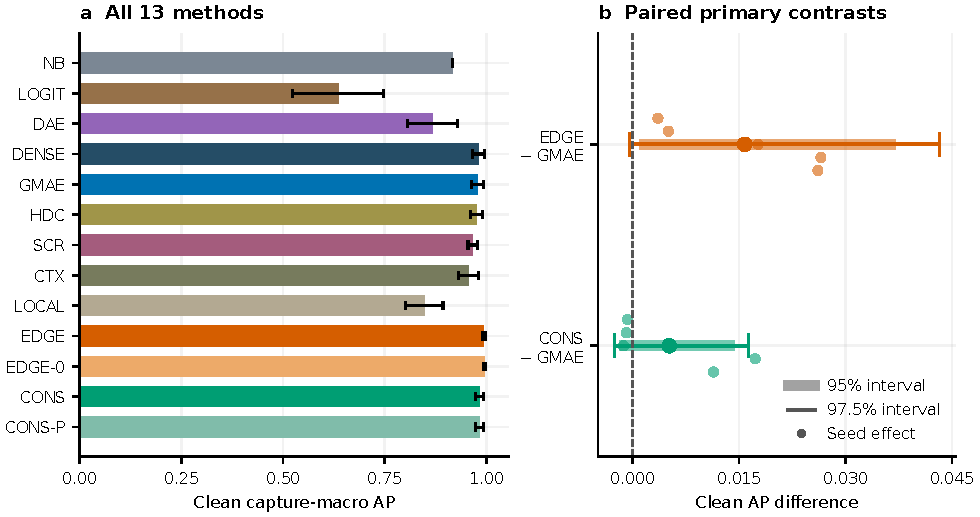
\includegraphics[width=\linewidth]{figures/fig1.pdf}
\caption{Clean performance and uncertainty. (A) Thirteen-method capture-macro AP with descriptive 95\% seed-t intervals. (B) Paired seed/time-block 95\% and 97.5\% intervals for the two specified contrasts. Both wider intervals cross zero; descriptive rankings do not establish superiority. Figure labels abbreviate EDGE\_GMAE, EDGE\_DENSE, CONS\_GMAE and CONS\_PRE as EDGE, EDGE-0, CONS and CONS-P; SCR, CTX and LOCAL omit the \_FLOW suffix.}
\end{figure}

EDGE\_DENSE, without pretraining, has the highest mean AP, 0.99500. GMAE also trails DENSE descriptively. Consequently, the gated family's clean gain cannot be credited to masked pretraining. EDGE\_GMAE's capture-specific AP improvements are 0.00079, 0.04242, and 0.00420; the largest is concentrated in capture 11. Capture conditions and malware family are confounded, so this pattern does not identify a family-specific causal mechanism.\par

Figure 2 separates capture-specific AP and pooled reliability. EDGE\_GMAE reduces Brier score from 0.05973 to 0.04262 and FPR from 0.07330 to 0.04265, while recall remains similar (0.81815 versus 0.81600). Prior shift makes frozen operating points consequential: LOGIT's FPR approaches one. Cheap NB exceeds DAE in AP, while contextual CTX\_FLOW exceeds LOCAL\_FLOW. These comparisons discourage assuming that more elaborate reconstruction or HDC augmentation necessarily helps.\par

\begin{figure}[tbp]
\centering
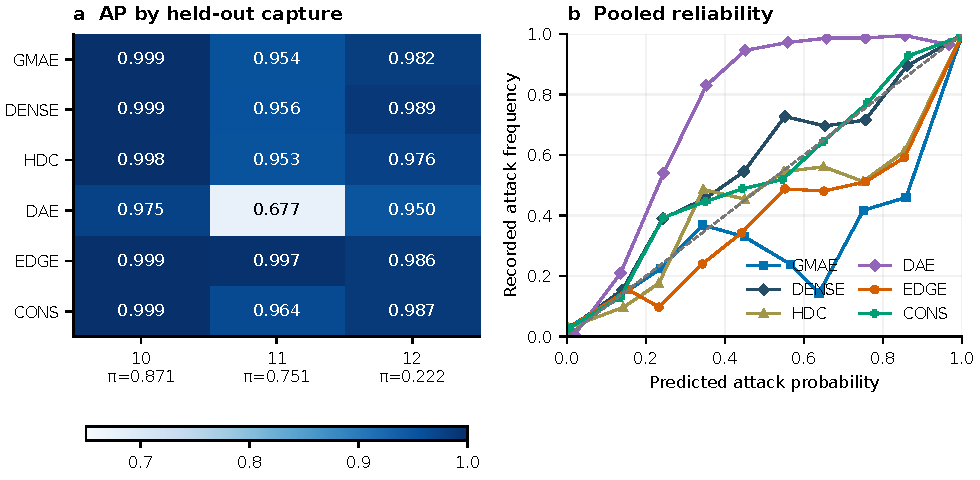
\includegraphics[width=\linewidth]{figures/fig2.pdf}
\caption{Capture-specific discrimination and pooled calibration. (A) Clean AP for GMAE, DENSE, HDC, DAE, EDGE\_GMAE, and CONS\_GMAE, showing variation across fixed test captures. (B) Clean reliability bins pooled by flow support across captures and seeds. Repeated predictions share flows and are not independent observations.}
\end{figure}

\subsection{Stress and matched controls}

At 50\% missingness, AP is 0.93553 for GMAE, 0.95962 for EDGE\_GMAE, 0.95360 for EDGE\_DENSE, and 0.95249 for CONS\_GMAE. At 40\% numeric replacement, values are 0.96716, 0.98535, 0.98432, and 0.97781, respectively (Figure 3). Thus gated pretraining has a descriptive advantage over its no-pretraining control under severe missingness, despite no clean advantage.\par

CONS\_GMAE's clean increment over CONS\_PRE is only 0.00076; CONS\_PRE is slightly higher under both missingness levels. The additional supervised consistency term therefore lacks a consistent descriptive benefit. These observations concern fixed artificial stresses, not robustness to adaptive adversaries.\par

\begin{figure}[tbp]
\centering
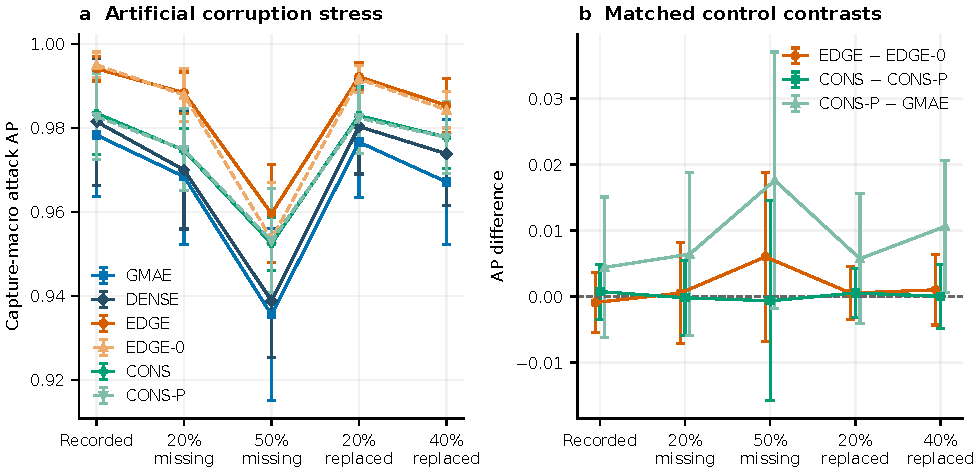
\includegraphics[width=\linewidth]{figures/fig3.pdf}
\caption{Artificial corruption and matched controls. (A) Capture-macro AP for six graph methods across five conditions. (B) Three pretraining/consistency contrasts, with descriptive seed-t intervals; CONS\_PRE versus GMAE jointly changes view count and alignment. Missing and replacement conditions alter features while retaining endpoint topology.}
\end{figure}

\FloatBarrier

\subsection{Resource costs and verification}

A common-session timing audit uses the same prepared 32-flow window for all thirteen inference architectures. Median bounded host-to-GPU-to-host latency is 2.374 ms for GMAE, 2.929 ms for EDGE\_GMAE, and 2.381 ms for CONS\_GMAE; corresponding p95 values are 2.805, 3.714, and 2.839 ms. EDGE's parameter-free gate adds computation and doubles incremental peak allocation from 0.093 to 0.187 MiB. CONS preserves inference architecture but increases mean training time from the historical GMAE measurement of 24.148 s to 29.994 s. Early stopping and separate training sessions prevent interpreting timings as controlled FLOP comparisons.\par

Timing includes decoded-input transfer, normalization, endpoint graph construction, inference, and prediction return. It excludes flow extraction, waiting for completion/windows, cold loading, and network transit. Incremental memory excludes resident model/data allocations. These are bounded processing costs, not complete detection latency or communication compression (Figure 4).\par

\begin{figure}[H]
\centering
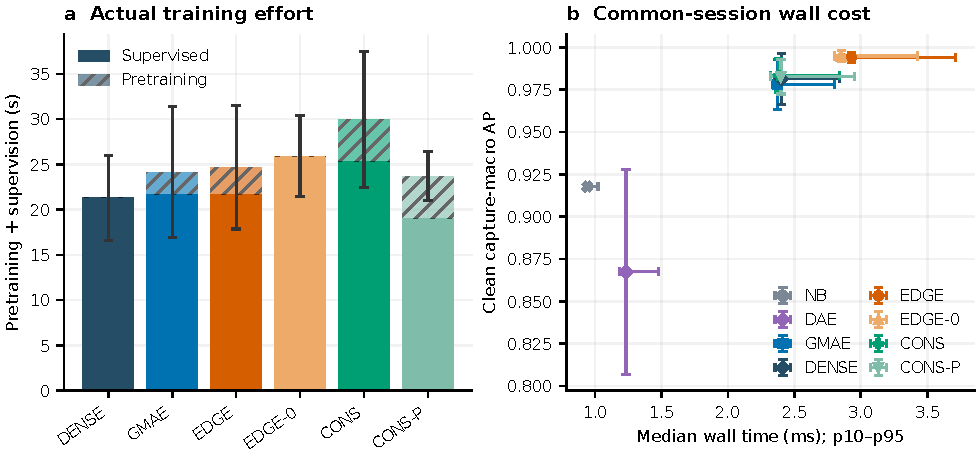
\includegraphics[width=\linewidth]{figures/fig4.pdf}
\caption{Measured computational tradeoffs. (A) Actual supervised and pretraining times for six graph methods; baseline training measurements are imported. (B) Common-session wall latency versus AP for eight methods, with p10–p95 repeat quantiles horizontally. Timing quantiles describe repeated measurements, not confidence intervals. Unequal forward passes and early stopping affect training cost.}
\end{figure}

Audits checked 975 summary records, 6,825 recomputed metrics, and 65 checkpoint hashes. Seventy-five replay cases for GMAE and the four new methods reproduced probabilities, AP, and Brier exactly. Training trajectories and seed effects appear in Figures S3–S4. These checks establish artifact consistency, not external validity.\par

\FloatBarrier

\section{Limitations and Scope}

Selected labels, recurring hosts, and reused historical test captures restrict generalization; newly reserved contemporary traffic from independent organizations would guide improvements in transferability.\par

Matched controls leave reconstruction and consistency contributions partly unresolved; a two-view zero-alignment control would isolate mechanisms and guide simpler, more effective training.\par

Retrospective flow classification leaves operational planning untested; sequential cyber testbeds would reveal how representation improvements affect replanning quality, mission utility, and communication costs.\par

\clearpage

\section{Conclusion}

We introduced and tested two telemetry-specific extensions of masked graph learning: parameter-free aggregation weighted by visible-feature overlap and compatibility, and latent and prediction consistency across masked views. Gated models achieved the highest observed mean average precision in every evaluated condition; consistency training improved the reference model's mean performance while preserving its inference architecture. Matched controls highlight aggregation as a productive design choice and reveal the condition-dependent contribution of masked pretraining. These exploratory findings provide tested mechanisms and measured computational tradeoffs to guide evidence regeneration and future integration with vector-symbolic and neurosymbolic cyber planning.\par

\section*{References}\begin{enumerate}[label={[\arabic*]},leftmargin=6mm,labelsep=1.5mm,itemsep=3pt,parsep=0pt,topsep=0pt]

\item Z. Hou, X. Liu, Y. Cen, Y. Dong, H. Yang, C. Wang, and J. Tang, “GraphMAE: Self-Supervised Masked Graph Autoencoders,” in Proc. ACM SIGKDD, 2022. \url{https://arxiv.org/abs/2205.10803}.

\item Z. Hou, Y. He, Y. Cen, X. Liu, Y. Dong, E. Kharlamov, and J. Tang, “GraphMAE2: A Decoding-Enhanced Masked Self-Supervised Graph Learner,” in Proc. ACM Web Conference, 2023. \url{https://arxiv.org/abs/2304.04779}.

\item W. Jin, Y. Ma, X. Liu, X. Tang, S. Wang, and J. Tang, “Graph Structure Learning for Robust Graph Neural Networks,” in Proc. ACM SIGKDD, 2020. \url{https://arxiv.org/abs/2005.10203}.

\item J. Han, W. Huang, Y. Rong, T. Xu, F. Sun, and J. Huang, “Structure-Aware DropEdge Towards Deep Graph Convolutional Networks,” IEEE Transactions on Neural Networks and Learning Systems, early access, 2023, doi:10.1109/TNNLS.2023.3288484.

\item S. Song, P. Li, M. Dun, Y. Zhang, H. Cao, and X. Ye, “Equipping Graph Autoencoders: Revisiting Masking Strategies from a Robustness Perspective,” in Proc. SIAM International Conference on Data Mining, 2025, pp. 366–375, doi:10.1137/1.9781611978520.39.

\item G. Tang, K. Liu, X. Yang, and Y. Qian, “Reconstruction Outcomes Look Similar but Processes Differ: Improving Context Consistency and Coverage in Graph Masked Auto-Encoder,” in Proc. ICML, PMLR, vol. 306, 2026, pp. 118954–118971. \url{https://proceedings.mlr.press/v306/tang26l.html}.

\item S. Laine and T. Aila, “Temporal Ensembling for Semi-Supervised Learning,” in Proc. International Conference on Learning Representations, 2017. \url{https://arxiv.org/abs/1610.02242}.

\item S. García, M. Grill, J. Stiborek, and A. Zunino, “An empirical comparison of botnet detection methods,” Computers \& Security, vol. 45, pp. 100–123, 2014, doi:10.1016/j.cose.2014.05.011. Dataset: \url{https://www.stratosphereips.org/datasets-ctu13}.

\item P. Vincent, H. Larochelle, Y. Bengio, and P.-A. Manzagol, “Extracting and Composing Robust Features with Denoising Autoencoders,” in Proc. International Conference on Machine Learning, 2008, pp. 1096–1103, doi:10.1145/1390156.1390294.

\item D. Kleyko, D. A. Rachkovskij, E. Osipov, and A. Rahimi, “A Survey on Hyperdimensional Computing aka Vector Symbolic Architectures, Part I: Models and Data Transformations,” ACM Computing Surveys, vol. 55, no. 6, pp. 1–40, 2022, doi:10.1145/3538531.

\item I. Loshchilov and F. Hutter, “Decoupled Weight Decay Regularization,” in Proc. International Conference on Learning Representations, 2019. \url{https://arxiv.org/abs/1711.05101}.

\item C. Guo, G. Pleiss, Y. Sun, and K. Q. Weinberger, “On Calibration of Modern Neural Networks,” in Proc. International Conference on Machine Learning, PMLR, vol. 70, 2017, pp. 1321–1330. \url{https://proceedings.mlr.press/v70/guo17a.html}.

\end{enumerate}

\end{document}
